\begin{figure}
\begin{center}
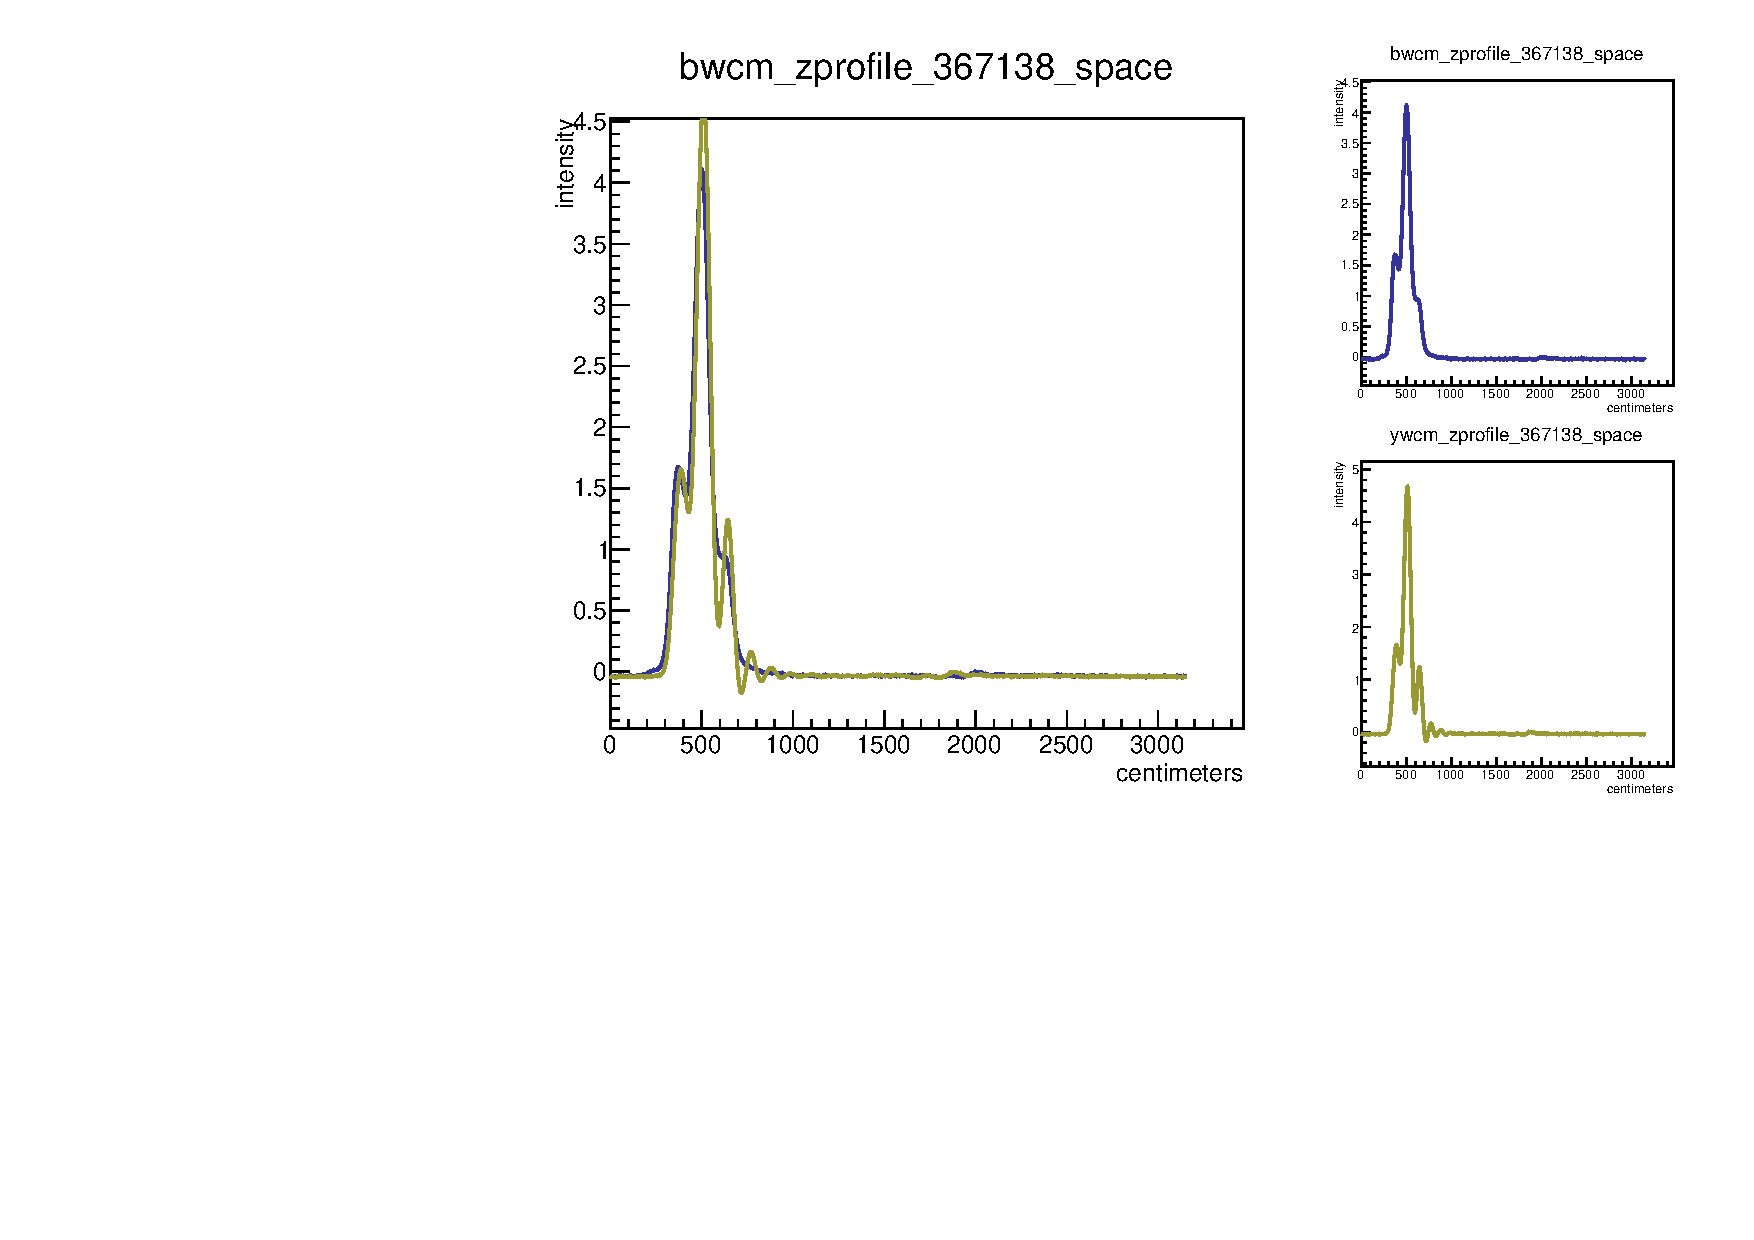
\includegraphics[width=\linewidth,height=\textheight,keepaspectratio]{../HourglassCorrection/figs/367138_wcm_zprofile}
\caption{ 
Left: the blue and yellow wall current monitor beam z-profiles. One can see the
three beam buckets which make up one so-called "filled bunch". Bunches are
approximately 1000 cm long, the entire profile passes the IR once every 106
nanoseconds, though most of the bunch is actually within a time envelope of
approximately 35 nanosecons. The panes on the right show the blue beam (top)
and the yellow beam (bottom).
}
\label{fig:367138_wcm_zprofile}
\end{center}
\end{figure}
